% ******************************* Lab report Template ***************************

\documentclass[a4paper,12pt,unnumberedsections,twoside]{Classes/LTJournalArticle}

% ******************************************************************************
% ******************************* Configurations ********************************
% ******************************************************************************

% ******************************************************************************
% Add spaces between paragraphs
%\setlength{\parskip}{0.5em}
% Ragged bottom avoids extra whitespaces between paragraphs
\raggedbottom
% To remove the excess top spacing for enumeration, list and description
%\usepackage{enumitem}
%\setlist[enumerate,itemize,description]{topsep=0em}

% *****************************************************************************
% ******************* Fonts (like different typewriter fonts etc.)*************

% *****************************************************************************
% **************************** Custom Packages ********************************

% **************************** ******Math *************************************
\usepackage{amsmath}

% ************************* Algorithms and Pseudocode **************************

%\usepackage{algpseudocode}


% ********************Captions and Hyperreferencing / URL **********************

% Captions: This makes captions of figures use a boldfaced small font.
\RequirePackage[tableposition=top]{caption}
%\DeclareCaptionFormat{custom}{#1#2\small #3}
\captionsetup{labelfont={sc,bf}, width=.9\textwidth}%format=custom, 
%\renewcommand{\figurename}{Fig.} %to support older versions of captions.sty


% *************************** Graphics and figures *****************************

%\usepackage{rotating}
%\usepackage{wrapfig}

% Uncomment the following two lines to force Latex to place the figure.
% Use [H] when including graphics. Note 'H' instead of 'h'
\usepackage{float}
%\restylefloat{figure}

% Subcaption package is also available in the sty folder you can use that by
% uncommenting the following line
% This is for people stuck with older versions of texlive
%\usepackage{sty/caption/subcaption}
\usepackage{subcaption}

% ********************************** Tables ************************************
\usepackage{booktabs} % For professional looking tables
\usepackage{multirow}
\usepackage{svg}
\usepackage{graphicx, import}

%\usepackage{multicol}
%\usepackage{longtable}
%\usepackage{tabularx}


% *********************************** SI Units *********************************
\usepackage{siunitx} % use this package module for SI units
\ifdefined\qty\else
	\ifdefined\NewCommandCopy
		\NewCommandCopy\qty\SI
	\else
		\NewDocumentCommand\qty{O{}mm}{\SI[#1]{#2}{#3}}
	\fi
	\fi
\ifdefined\unit\else
	\ifdefined\NewCommandCopy
		\NewCommandCopy\unit\si
	\else
		\NewDocumentCommand\unit{O{}m}{\si[#1]{#2}}
	\fi
\fi



% ******************************* Line Spacing *********************************

% Choose linespacing as appropriate. Default is one-half line spacing as per the
% University guidelines

% \doublespacing
% \onehalfspacing
% \singlespacing


% ************************ Formatting / Footnote *******************************

% Don't break enumeration (etc.) across pages in an ugly manner (default 10000)
%\clubpenalty=500
%\widowpenalty=500

%\usepackage[perpage]{footmisc} %Range of footnote options


% *****************************************************************************
% *************************** Bibliography  and References ********************

%\usepackage{cleveref} %Referencing without need to explicitly state fig /table

\usepackage[backend=biber]{biblatex}
% changes the default name `Bibliography` -> `References'

\usepackage{listings}
\lstdefinestyle{mystyle}{
	backgroundcolor=\color{backcolour},   
	commentstyle=\color{codegreen},
	keywordstyle=\color{magenta},
	numberstyle=\tiny\color{codegray},
	stringstyle=\color{codepurple},
	basicstyle=\ttfamily\footnotesize,
	breakatwhitespace=false,         
	breaklines=true,                 
	captionpos=b,                    
	keepspaces=true,                 
	numbers=left,                    
	numbersep=5pt,                  
	showspaces=false,                
	showstringspaces=false,
	showtabs=false,                  
	tabsize=2
}
% ******************************************************************************
% ************************* User Defined Commands ******************************
% ******************************************************************************

% *********** To change the name of Table of Contents / LOF and LOT ************

%\renewcommand{\contentsname}{My Table of Contents}
%\renewcommand{\listfigurename}{My List of Figures}
%\renewcommand{\listtablename}{My List of Tables}


% ********************** TOC depth and numbering depth *************************

\setcounter{secnumdepth}{2}
\setcounter{tocdepth}{2}


% ******************************* Nomenclature *********************************

% To change the name of the Nomenclature section, uncomment the following line

%\renewcommand{\nomname}{Symbols}


% ********************************* Appendix ***********************************

% The default value of both \appendixtocname and \appendixpagename is `Appendices'. These names can all be changed via:

%\renewcommand{\appendixtocname}{List of appendices}
%\renewcommand{\appendixname}{Appndx}

% *********************** Configure Draft Mode **********************************

% Uncomment to disable figures in `draft'
%\setkeys{Gin}{draft=true}  % set draft to false to enable figures in `draft'

% These options are active only during the draft mode
% Default text is "Draft"
%\SetDraftText{DRAFT}

% Default Watermark location is top. Location (top/bottom)
%\SetDraftWMPosition{bottom}

% Draft Version - default is v1.0
%\SetDraftVersion{v1.1}

% Draft Text grayscale value (should be between 0-black and 1-white)
% Default value is 0.75
%\SetDraftGrayScale{0.8}


% ******************************** Todo Notes **********************************
%% Uncomment the following lines to have todonotes.

%\ifsetDraft
%	\usepackage[colorinlistoftodos]{todonotes}
%	\newcommand{\mynote}[1]{\todo[author=kks32,size=\small,inline,color=green!40]{#1}}
%\else
%	\newcommand{\mynote}[1]{}
%	\newcommand{\listoftodos}{}
%\fi

% Example todo: \mynote{Hey! I have a note}


\addbibresource{References/references.bib}

%\runninghead{} % A shortened article title to appear in the running head, leave this command empty for no running head

%\footertext{\textit{} % Text to appear in the footer, leave this command empty for no footer text

\setcounter{page}{1} % The page number of the first page, set this to a higher number if the article is to be part of an issue or larger work

\title{Electroosmotic Flow and Electrophoresis} % Article title, use manual lines breaks (\\) to beautify the layout

\author{%
	Niklas Scheuler, Niklas Müller and Jonas Scheunemann
}

\renewcommand{\maketitlehookd}{%
	\begin{abstract}
		\noindent Empty abstract.
	\end{abstract}
}


\begin{document}


\maketitle

% *********************** Adding TOC  ***********************

\tableofcontents

% \printnomenclature[space] space can be set as 2em between symbol and description
%\printnomenclature[3em]

% ******************************** Main Matter *********************************

%%!TEX root = ../Lab_report.tex
%*******************************************************************************
%*********************************** Theory Chapter *****************************
%*******************************************************************************
\section{Theory}
\subsection{Lattice-Boltzmann method}
The Boltzmann equation describes the statistical behavior of a thermodynamic system out of equilibrium. It is given by:

\begin{equation}\label{eq:boltzmann-transport}
\frac{\partial f}{\partial t} + \mathbf{v} \cdot \nabla_{\mathbf{r}} f + \mathbf{F} \cdot \nabla_{\mathbf{v}} f = \left( \frac{\partial f}{\partial t} \right)_{\text{coll}}
\end{equation}

where \( f = f(\mathbf{r}, \mathbf{v}, t) \) is the distribution function, \( \mathbf{r} \) is the position, \( \mathbf{v} \) is the velocity, \( \mathbf{F} \) is the external force and \( \left( \frac{\partial f}{\partial t} \right)_{\text{coll}} \) is the collision term.

The Bhatnagar-Gross-Krook (BGK) approximation simplifies the collision term to 

\begin{equation}\label{eq:collision}
\left( \frac{\partial f}{\partial t} \right)_{\text{coll}} = -\frac{1}{\tau} (f - f^{\text{eq}})
\end{equation}
where \( \tau \) is the relaxation time and \( f^{\text{eq}} \) is the local equilibrium distribution function. We assume that there is a equilibrium distribution to which the system relaxes. How fast this equilibrium is reached is encoded in the relaxation time $\tau$, which corresponds directly to the viscosity of the fluid.\\

The Ansatz for the Lattice Boltzmann Method (LBM) is now to discretise the position space and form a lattice as well as discretising the time. The distributions are then also discretised, with each lattice site having the number of distributions corresponding to neighbouring sites. This number of neighbours depends on the lattice model used. So for each time step the collision is calculated with \autoref{eq:collision} for each of the different distributions $f_i$ on a single lattice site. Then the streaming to the other lattice sites is calculated using the final form of the approximation of \autoref{eq:boltzmann-transport}

\begin{equation}
f_i(\mathbf{r} + \mathbf{e}_i \Delta t, t + \Delta t) = f_i(\mathbf{r}, t) + \frac{\Delta t}{\tau} \left( f_i^{\text{eq}}(\mathbf{r}, t) - f_i(\mathbf{r}, t) \right)
\end{equation}

Advantages of the LBM are the high parralisability of the computations, resulting in short simulation times, and the efficient simulation of multi-phase fluids.
Disadvantages are the high memory consumption and the fact that LBM can't calculate fluids with a high Mach number meaning compressible flows.



\subsection{Particle-Particle - Particle-Mesh}

The P3M algorithm, also known as the Particle-Particle Particle-Mesh method, is a computational approach utilized for efficient computation of long-range interactions in systems with periodic boundary conditions. This method is particularly useful in molecular dynamics simulations.

\subsubsection{Ewald summation}
Ewald summation is a technique used to compute non-neglectable long-range interactions in periodic systems by splitting the potential into short-range and long-range components. Looking at a charge distribution of a Coulomb potential with 
\begin{equation}
\rho = \sum_{\mathbf{n} \in \mathbb{L}^3} \sum_{i=1}^{N} q_i \delta(\mathbf{r} - \mathbf{r}_i - \mathbf{n})
\end{equation}
we can add a gaussian shielding charge of the form
$ \rho_{\text{Gauss}}(\mathbf{r}) = \left( \frac{\alpha}{\sqrt{\pi}} \right)^3 e^{-\alpha^2 r^2}$ 
for each charged particle  with a width $a$, turning the delta function into
\begin{equation}
\delta(\mathbf{r}) = \rho_{\text{Gauss}}(\mathbf{r})+ {[\delta(\mathbf{r}) - \rho_{\text{Gauss}}(\mathbf{r})]}.
\end{equation}

The potential for the Coulomb Ewald Summation can now be written with a real space, k-space and a self-interaction part
\begin{equation}
  U = U^{r} + U^{k} + U^{s}
\end{equation}

\begin{align*}
  U^{r} &= \frac{l_B}{2} \sum_{\mathbf{m} \in \mathbb{Z}^3} \sum_{i,j}' \frac{q_i q_j \, \text{erfc}(\alpha | \mathbf{r}_{ij} + \mathbf{m}L |)}{| \mathbf{r}_{ij} + \mathbf{m}L |}  \\
  U^{k} &= \frac{l_B}{2L^3} \sum_{\mathbf{k} \neq 0} \frac{4\pi}{k^2} e^{-k^2 / 4\alpha^2} |\hat{\rho}(\mathbf{k})|^2 \\
  U^{s} &= -\frac{\alpha l_B}{\sqrt{\pi}} \sum_{i} q_i^2\\
\end{align*}

\subsubsection{P3M algorithm steps}
The idea of the P3M algorithm is now to speed up the reciprocal space calculations by calculating them on a grid.
So for the first step we need to transform the charges onto a mesh. 
This is done with 
\begin{equation}
  \rho_M(\mathbf{r}_p) = \frac{1}{h^3} \sum_{i=1}^{N} q_i W^{p}(\mathbf{r}_p - \mathbf{r}_i)
\end{equation}
where $W^{p}(\mathbf{r}_p - \mathbf{r}_i)$ are cardinal B-Splines.
With the mesh initialized we need ot obtain the fourier transformed charge distribution $\hat{\rho}(k)$, so we can solve the Poisson equation with
\begin{equation}
  \hat{\phi}(k) = G(k)\hat{\rho}(k)
\end{equation}
where $G(k)$ is the optimal influence function.
With this it is only a matter of obtaining the field by differentiation in Fourier space $ik\hat{\phi}(k) = \hat{E}(k)$, transforming back to real space  and interpolating the field at position of charges to get the forces for the MD calculations. 

%%!TEX root = ../Lab_report.tex
%*******************************************************************************
%*********************************** Methods Chapter *****************************
%*******************************************************************************
\section{Methods}

%********************************** %First Section  **************************************



%!TEX root = ../Lab_report.tex
%*******************************************************************************
%*********************************** Analysis Chapter *****************************
%*******************************************************************************
\section{Free-Solution DNA electrophoresis}
Electrophoresis is an experimental technique used to separate charged molecules like polyelectrolyte chains by making use of the interaction between the particles and external electric fields. In a solution with counterions, the dynamics of a charged polymer chain is governed by electrostatic interactions between polymers and counterions as well as hydrodynamic interactions. We investigate the dynamical properties of polyelectrolytes of different lengths in a bulk solution using coarse grained Molecular Dynamics simulations with electrostatics and hydrodynamical interactions. All simulations were carried out with ESPResSo \cite{weik2019espresso}. Electrostatic interactions are modelled efficiently with the P3M method with periodic boundary conditions. The Lattice-Boltzmann method (LBM) is employed to model hydrodynamical interactions.

\subsection{System setup}
We conducted several simulations of a system with equal parameters except the number of monomers $N$ on the polyelectrolyte chain. In every simulation the system consisted of $N$ (where $1\le N \ge 32$)monomers connected by bonded interactions modelled with a FENE potential. Furthermore, $N$ counterions are placed at random positions in the simulation box. All simulated particles exhibited short ranged repulsive interactions, modelled by a WCA potential and long ranged electrostatic interactions, where a Bjerrum length of $l_\text{B} = 2.84$ in reduced units was chosen. The box size of the cubic simulation box was chosen such that the mean concentration of monomers in the solution was kept constant at $\SI{5}{\milli M}$. To remove overlap between all particles in the system, first, a total of $2000$ gradient based energy minimization steps were performed to remove overlap between all particles in the system. Subsequently, after activating electrostatic and hydrodynamic interactions, the system was equilibrated for $\SI{5e5}{}$ integration steps. During the production run, we sampled data every integration step for a total of $\SI{5e6}{}$ steps. Figure \ref{fig:vmd} displays the simulated system for one simulation with $N=32$ after equilibration.
\begin{figure}[H]
	\centering
	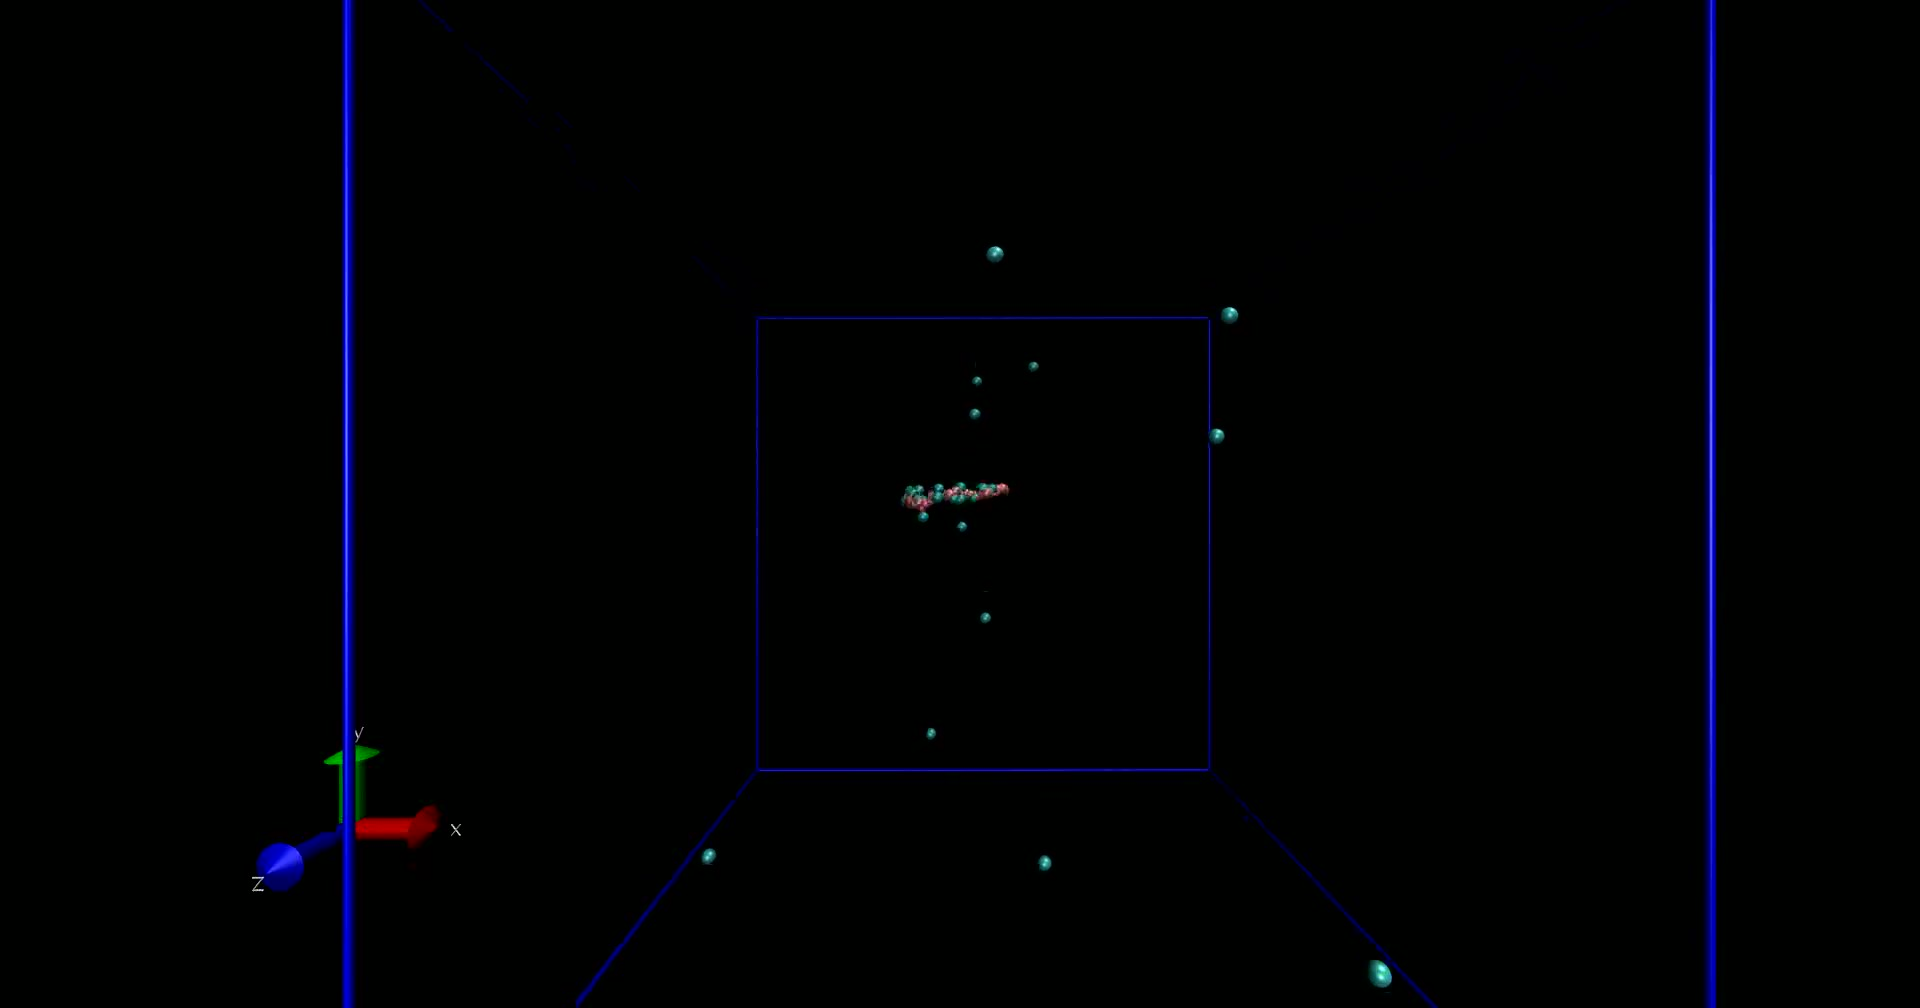
\includegraphics[width=\columnwidth]{Analysis_1/VMD_visualization}
	\captionsetup{width=\columnwidth}
	\caption{Visualization of a simulated polyelectrolyte with a chain length of 32.}
	\label{fig:vmd}
\end{figure}
%!TEX root = ../Lab_report.tex

Next to the diffusion coefficient $D$, the electrophoretic mobility $\mu$ is an important transport coefficient of the system. It describes the motion of a polyelectrolyte chain in the presence of an external field. It is simply defined by
\begin{align}
	\mu = \frac{v}{E},
\end{align}
where $v$ is the average velocity of the polymer chain and $E$ is the applied external field. Since the system is simulated at very small time scales, it is difficult to separate the motion of the polymer that is caused by the external from diffusive motions. Therefore, an alternative definition of the electrophoretic mobility will be useful. For weak electric fields the Green-Kubo relation
\begin{align}
	\label{eq:mu}
	\mu = \frac{1}{3k_\text{B}T} \sum_{i} q_i \int_{0}^{\infty} \langle \vec{v}_i(0) \cdot \vec{v}_\text{cm}(\tau) \rangle d\tau,
\end{align}
where $i$ denotes single particles in the system (monomers and counterions) and $\vec{v}_i$ and $q_i$ their respective velocity and charge. Importantly, the mobility can also be computed from trajectories in the absence of an external electric field when using the definition given in Equation \eqref{eq:mu}.
\begin{figure}[H]
	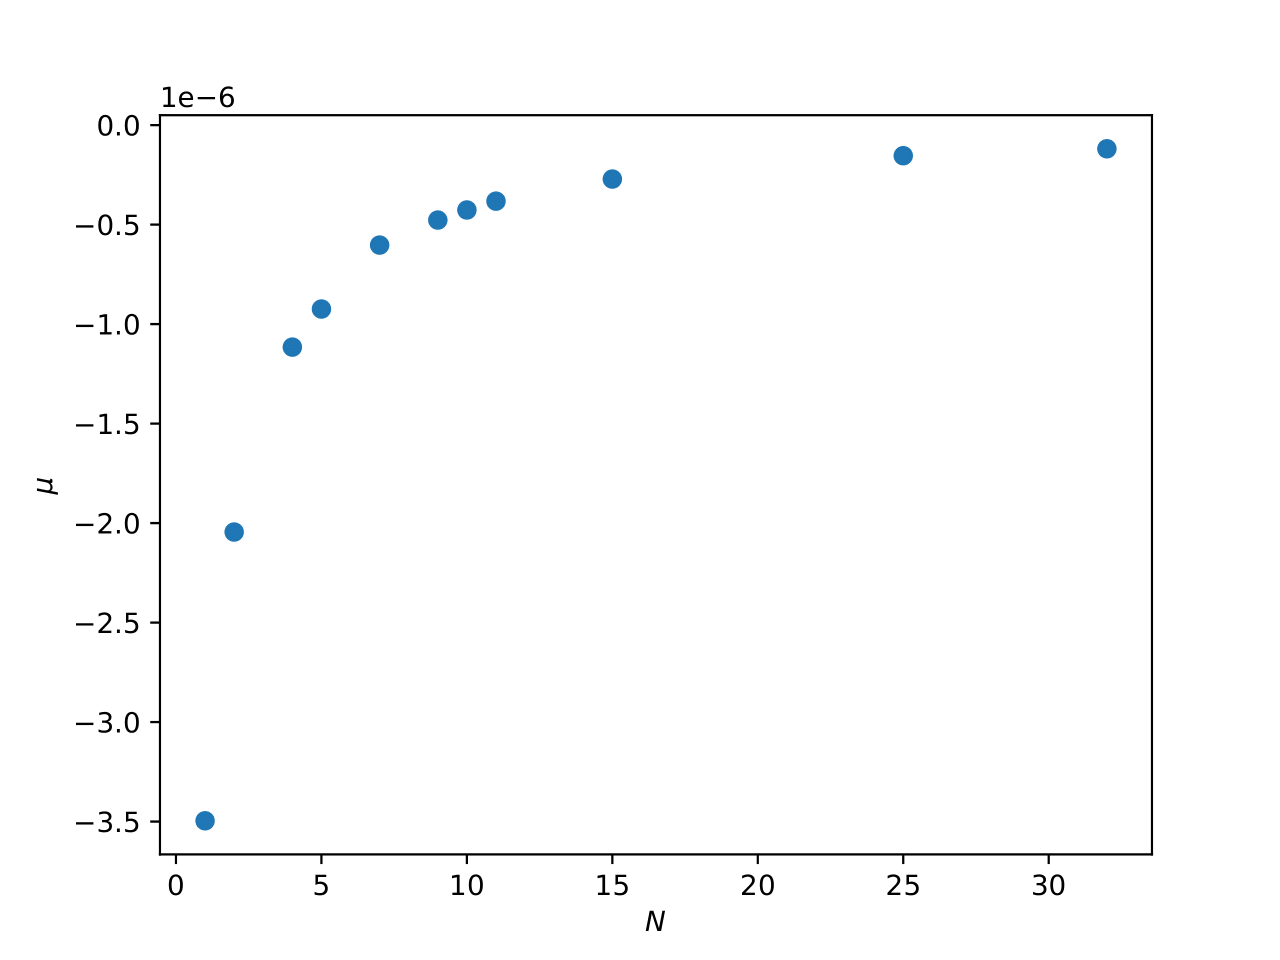
\includegraphics[width=\columnwidth]{Analysis_1/test_mobilities}
	\captionsetup{width=\columnwidth}
	\caption{Calculated mobilities of polymers as a function of chain length from MD simulations.}
	\label{fig:mobilities}
\end{figure}
The observed mobilities are in disagreement with the expected behaviour. The monotonic increase of $\mu$ with the number of monomers is only expected for short polymers. In general, in the steady state, the electric force on the polymer $\vec{F}_E = Q_\text{eff} \vec{E}$ is balanced by the counteracting solvent drag force $\vec{F}_D = -\Gamma_\text{eff} \vec{v}$. The experimentally observed constant mobility for long chains can be explained with the free draining-picture. The polymer is assumed to be penetrated by counterions, which drag along surrounding solvent. This results in the destruction of long range hydrodynamical interactions. The effective friction on the polymer scales linearly with the number of monomers for long chains, i.e.
\begin{equation}
	\Gamma_\text{eff} = \Gamma N.
\end{equation}
Together with the effective charge predicted by Manning theory of
\begin{equation}
	Q_\text{eff} = N / \xi
\end{equation}
a constant mobility
\begin{equation}
	\mu = \frac{v}{E} = \frac{Q_\text{eff}}{\Gamma_\text{eff}} = \frac{N}{\Gamma N \xi} = \frac{1}{\Gamma \xi}
\end{equation}
is obtained. In the transition region between short and long chains a mobility maximum is expected. Our results indicate an inaccurate description of hydrodynamic interaction in the system, which could be the reason for the unexpected behavior of the mobility.
%%!TEX root = ../Lab_report.tex
%*******************************************************************************
%*********************************** Additional sections for analysis Chapter *****************************
%*******************************************************************************

\section{Electro-Osmotic flow}
Electro-Osmotic flow plays a crucial role in various scientific and industrial processes, especially in microfluidics, electrochemistry, and environmental science. In this work, the electro-osmotic flow of ions in a solution within a charged slit pore is investigated. We take a closer look at the density distribution of the ions as well as the flow profile of the solvent.
\subsection{System setup}
A snapshot of the system is shown in Figure \ref{fig:system1}. It consists of two infinite, parallel, charged walls with ions and a solvent in between. The ions are accelerated by an electric field.  In order to reduce the degrees of freedom, the solvent is represented by an Lattice-Boltzmann Fluid. The wall charge is represented by 64 charged particles with the charge $q=\text{e}$ that are fixed on each wall. They create an electric field that is homogeneous enough for our application. To keep the system electrically neutral, 128 counter ions are placed between the walls. Periodic boundary conditions are used in the plane  parallel to the walls.  The electrostatic interactions are solved by the ELC algorithm. Additionally all particles interact with each other and the walls via the Weeks-Chandler-Andersen potential. The simulation is performed with ESPResSo. A list with the system parameters can be found in the Appendix in Table \ref{tab:params}.
The python code can also be found in the Appendix. In the production runs, the simulations were always executed for 100000 integration steps and a step size $\Delta t= 0.01\,[t]$. Since the sampling of the flow and the density profile is numerically costly, only  every hundredth data point of the flow and the density profile was sampled.
\begin{figure}[H]
	\centering
	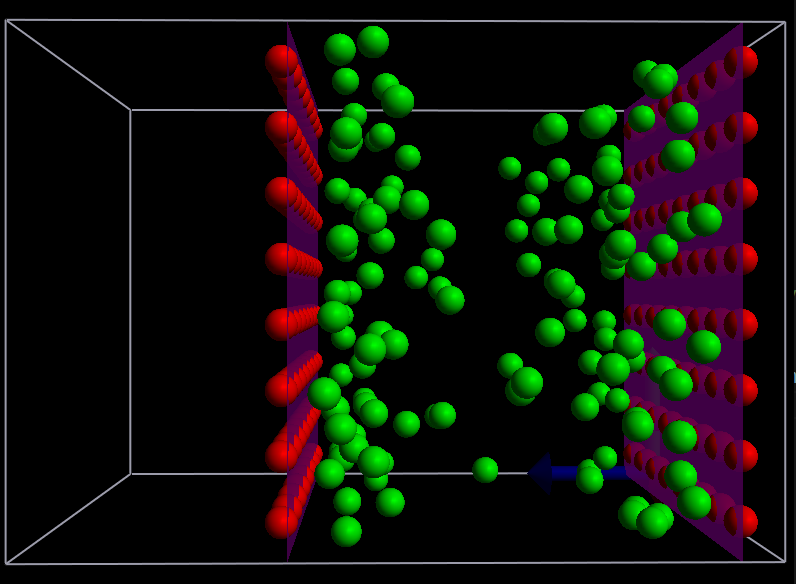
\includegraphics[width=\columnwidth]{Analysis_2/system}
	\captionsetup{width=\columnwidth}
	\caption{Visualization of the slit pore system. The wall charges (counter ions) are represented by red (green) spheres. The ELC gap is clearly visible on the left hand side of the left hand wall.}
	\label{fig:system}
\end{figure}
\subsection{Results}
The flow profile of the solvent is a characteristic observable of a system with electro-osmotic flow. As explained in section \ref{ } it can be calculated analytically in the continuum limit. The analytical solution yields a flat profile. This profile is highest at the center and goes to zero at the boundary. Figure \ref{fig:slit_plot} shows the flow profile obtained by the simulation as well as the theoretical curve. It can be seen that there is a good agreement.

\begin{figure}[H]
	\centering
	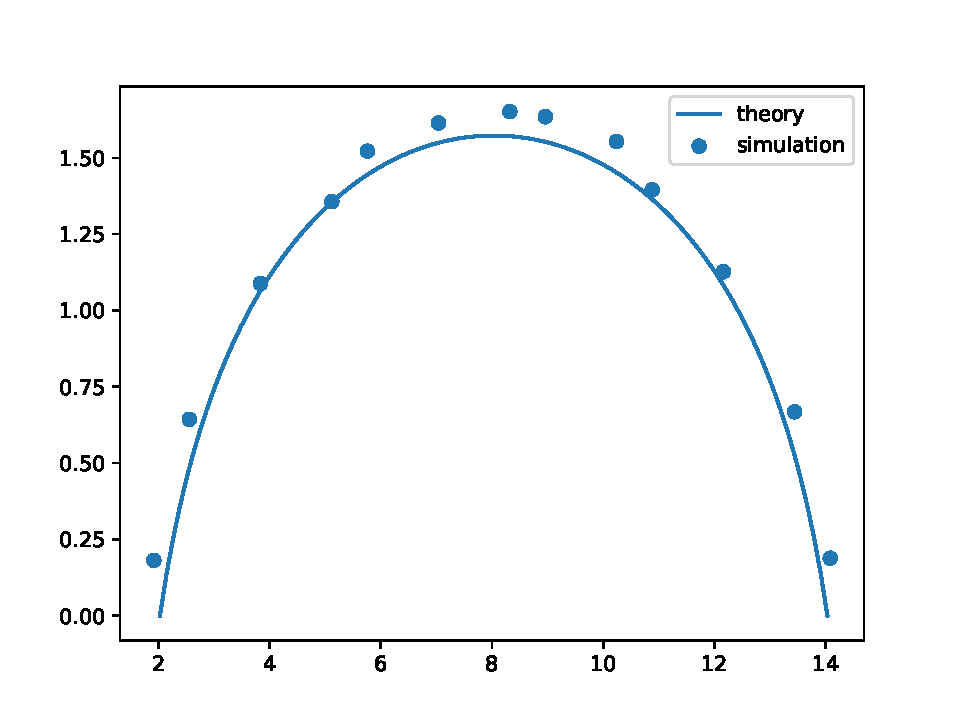
\includegraphics[width=\columnwidth]{slit_pore/prodrun_figs/fp}
	\captionsetup{width=\columnwidth}
	\caption{Comparison of the simulation data and the theoretical calculations of the flow profile.}
	\label{fig:slit_plot}
\end{figure}

Another interesting observable is the ion density profile. It can also be calculated in the continuum limit. Due to the opposing charge of the wall and the ions, they attract each other. Therefore, the ions accumulate close to the boundary. Due to the repulsion between  the ions, not all of the ions condensate at the wall. This behavior can be seen in Figure \ref{fig:slit_plot2}
\begin{figure}[H]
	\centering
	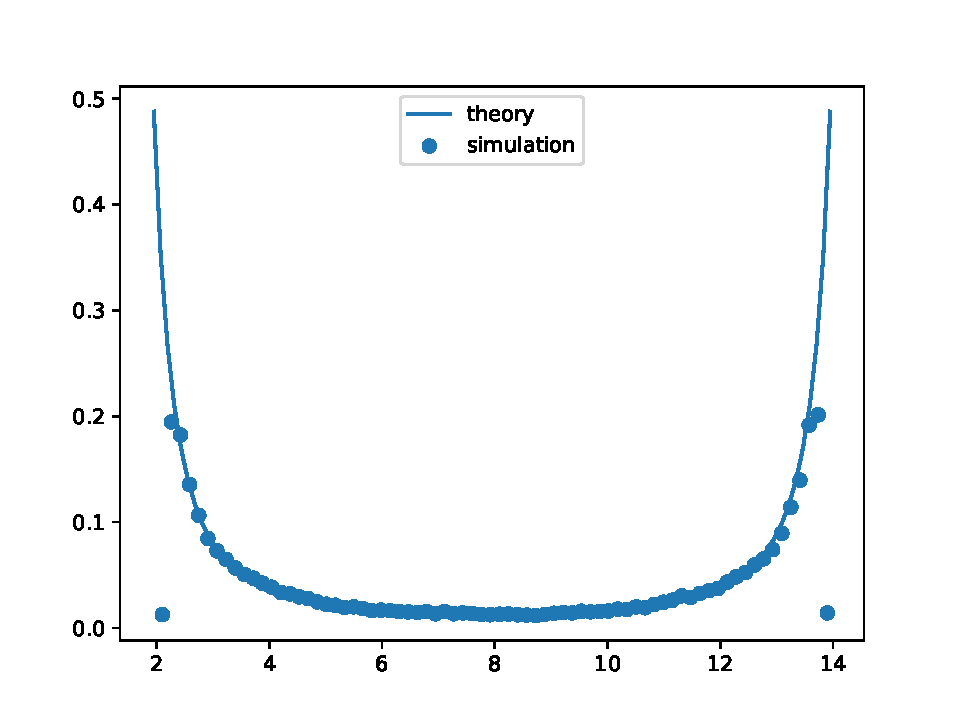
\includegraphics[width=\columnwidth]{slit_pore/prodrun_figs/id}
	\captionsetup{width=\columnwidth}
	\caption{Comparison of the simulation data and the theoretical calculations of the ion density.}
	\label{fig:slit_plot2}
\end{figure}
\begin{table}[H]
	\caption{System parameter in SI units and simulation units}
	\centering
	\begin{tabular}{l c c c c c}
		\toprule
		parameter  & value (SI units) & value (simulation units)\\
		\midrule
		channel width $d$&\SI{12}{nm}&12[x]\\
		counter ion charge $q$&\SI{1}{e}&1[q]\\
		thermal energy $k_{\text{B}}T$&$k_{\text{B}}\SI{300}{K}$&1[E]\\
		vacuum permittivity $\varepsilon_\text{0}$&\SI{8.85e-10}{s^2kgm^3}&\SI{1.428e-3}{}$[q]^2[t]^2/[m][x]^3$\\
		relative solvent permittivity5  $\varepsilon_\text{r}$&\SI{78.54}{}&78.54\\
		external electrical field $E$&\SI{0.646e9}{Vm^{-1}}&$25[E]/[q][x]$\\
		solvent density $\rho$&\SI{1000}{kg\per m^3}&$26.18[m]/[x]^3$\\
		kinematic solvent viscosity $\nu$&\SI{8.23e-8}{m^2\per s}&$0.25[x]^2/[t]$\\
		counterion frictional coefficient $\gamma$&\SI{1.910}{kg\per s}&15[m]/[t]\\
		\bottomrule
	\end{tabular}	
	\label{tab:params}
\end{table}

%%!TEX root = ../Lab_report.tex
%*******************************************************************************
%*********************************** First Chapter *****************************
%*******************************************************************************

\chapter{Results}  %Title of the Third Chapter

%********************************** %First Section  **************************************

%!TEX root = ../Lab_report.tex
\onecolumn
\lstset{basicstyle=\footnotesize\ttfamily, breaklines=true}
\section{Appendix}
\subsection{Polymer simulation script}
In the following, the \texttt{Python} script for the simulation of the polymer electrophoresis is given. \\
First, the required features from the \texttt{espressomd} package are imported and global constants for the physical system are set. 
\begin{lstlisting}[language=python]
import argparse
import espressomd
import espressomd.lb
import espressomd.version
import espressomd.electrostatics
import espressomd.observables
import espressomd.accumulators
import espressomd.polymer
import espressomd.visualization
import numpy as np
import logging
import pickle
import time
import tqdm
import matplotlib.pyplot as plt
import espressomd.io.writer.vtf
from itertools import repeat

logging.basicConfig(level=logging.INFO)

required_features = ["LENNARD_JONES"]
espressomd.assert_features(required_features)

parser = argparse.ArgumentParser(epilog=__doc__)
parser.add_argument('-n', '--num_monomer', type=int, required=True)
parser.add_argument('-steps', '--sim_steps', type=int, required=True)
parser.add_argument('-gamma', '--gamma_lb', type=float, required=False, default=20.)
parser.add_argument('-write_to_vtf', type=bool, required=False, default=False)
parser.add_argument('-p3m_eq_steps', type=int, required=False, default=1000000)
parser.add_argument('-e_field', type=bool, required=False, default=False)
args = parser.parse_args()

N_MONOMER = args.num_monomer
TOTAL_TIME_STEPS = args.sim_steps
EQULIBRATION_STEPS = int(1e6)
P3M_EQ_STEPS = args.p3m_eq_steps
WRITE_TO_VTF = args.write_to_vtf
GAMMA = args.gamma_lb
E_FIELD = 0.1 if args.e_field else 0.
logging.info(f"Setting external E-field of {E_FIELD}.")
DENSITY = 5e-5
SIGMA = 1. # 2.5 Angstrom
BOX_L = np.power((N_MONOMER / DENSITY), 1.0 / 3.0) * np.ones(3)
BOX_L = np.round(BOX_L)
L_BJERRUM = 2.84 # 7.1 Angstrom
# L_BJERRUM = 2.0 # 7.1 Angstrom
DELTA_T = 0.01
SEED = 42
\end{lstlisting}
Subsequently, functions are defined for building the system box, the polymer and the counterions. The function \texttt{equilibrate\_polymer} is responsible for removing overlaps after the insertion of new particles in the system.
\begin{lstlisting}[language=python]
def time_it(func):
	# Simple wrapper to measure the execution time of different functions.
	def wrapper(*args, **kwargs):
		start_t = time.perf_counter()
		func(*args, **kwargs)
		print(f"Function {func.__name__} took {time.perf_counter() - start_t:.2f}s to execute.")
	return wrapper

def build_system():
	system = espressomd.System(box_l=BOX_L)
	system.periodicity = [True, True, True]
	system.cell_system.skin = 0.4
	system.time_step = DELTA_T
	logging.info(f"Created Simulation with {N_MONOMER} monomers and box length L={BOX_L}.")
	system.non_bonded_inter[0, 0].wca.set_params(epsilon=0.25, sigma=1.0)
	system.non_bonded_inter[0, 1].wca.set_params(epsilon=0.25, sigma=1.0)
	system.non_bonded_inter[1, 1].wca.set_params(epsilon=0.25, sigma=1.0)
	return system

def build_polymer(system, n_monomers, fene, seed):
	polymer_pos = espressomd.polymer.linear_polymer_positions(n_polymers=1, beads_per_chain=n_monomers, seed=seed, bond_length=0.91, min_distance=0.9, start_positions=np.expand_dims(BOX_L/2., 0))
	p_previous = None
	for pos in polymer_pos[0]:
		p = system.part.add(pos=pos, type=0, q=-1)
		if p_previous is not None:
			p.add_bond((fene, p_previous))
	p_previous = p

def equilibrate_polymer(system,seed):
	logging.info("Removing overlaps of polymers...")
	print("BEFORE MINIMIZATION", system.analysis.energy()["total"])
	system.integrator.set_steepest_descent(
		f_max=0,
		gamma=10.,
		max_displacement=0.01)
	logging.info("Desired F_max polymers and counterions=" +str(FMAX))
	FMAX = 10
	system.integrator.run(1000)
	print("AFTER MINIMIZATION", system.analysis.energy()["total"])
	logging.info("F_max polymers is " + str(np.abs(system.part.all().f).max()))
	system.integrator.set_vv()
	logging.info("Remove overlap polymer finished.")
	logging.info("Equilibration polymer ...")
	system.thermostat.set_langevin(kT=1.0, gamma=1.0, seed=seed)
	system.integrator.run(20000)
	system.thermostat.turn_off()
	# system.galilei.kill_particle_motion()
	# system.galilei.galilei_transform()
	logging.info("F_max polymers"+str(np.abs(system.part.all().f).max()))
	logging.info("Equilibration polymer finished.")

def generate_counterions(system, n_counter_ions, seed):
	logging.info("Creating Counterions ...")
	# Spawn counterions closer around polymer
	com_polymer = system.part.select(type=0).pos.mean(0)
	counter_ions_pos = ((np.random.rand(n_counter_ions, 3) * 2) - 1) * BOX_L/ 2 + com_polymer
	# counter_ions_pos = np.random.rand(n_counter_ions, 3) * BOX_L
	for pos in counter_ions_pos:
		system.part.add(pos=pos, q=1., type=1)
	FMAX = 10
	logging.info("Removing overlap Counterions ...")
	print("BEFORE MINIMIZATION", system.analysis.energy()["total"])
	system.integrator.set_steepest_descent(
	f_max=0,
	gamma=30.,
	max_displacement=0.01)
	system.integrator.run(1000)
	print("AFTER MINIMIZATION", system.analysis.energy()["total"])
	logging.info("Desired F_max polymers and counterions="+str(FMAX))
	logging.info("F_max polymers and counterions is " + str(np.abs(system.part.all().f).max()))
	logging.info("Equilibration with counterions")
	logging.info("Remove overlap finished.")
	logging.info("Equilibration ...")
	system.integrator.set_vv()
	system.thermostat.set_langevin(kT=1.0, gamma=1.0, seed=seed)
	system.integrator.run(20000)
	system.thermostat.turn_off()
\end{lstlisting}		
After the insertion of all particles to the system, electrostatic and hydrodynamic interactions are activated and the system is equilibrated.
\begin{lstlisting}[language=python]
def turn_on_e_field(system):
	system.part.select(q=-1).ext_force = [0, 0, -E_FIELD]
	system.part.select(q=1).ext_force = [0, 0, E_FIELD]
	logging.info(f"Turned on E-field of {E_FIELD}.")

def turn_on_electrostatics(system, l_bjerrum, seed):
	if espressomd.version.minor() == 2:
		logging.info("P3m with GPU acceleration turned on.")
		p3m = espressomd.electrostatics.P3MGPU(prefactor=l_bjerrum, accuracy=0.0001)
		system.actors.add(p3m)
	else:
		logging.info("P3m with NO GPU acceleration turned on.")
		p3m = espressomd.electrostatics.P3M(prefactor=l_bjerrum, accuracy=0.0001)
		system.electrostatics.solver = p3m
	logging.info("Equilibration ...")
	system.thermostat.set_langevin(kT=1.0, gamma=1.0, seed=seed)
	for _ in tqdm.tqdm(range(P3M_EQ_STEPS), desc="Equilibrating electrostatics..."):
		system.integrator.run(1)
	system.thermostat.turn_off()

def set_hydrodynamic_interaction_walberla(system, seed, gamma):
	logging.info("Set hydrodynamic interactions Walberla.")
	system.galilei.kill_particle_motion()
	system.galilei.galilei_transform()
	lb=espressomd.lb.LBFluidWalberlaGPU(
		agrid=1.0, density=0.864, kinematic_viscosity=3.0, tau=system.time_step, kT=1, ext_force_density=[0.0,0.0,0.0], seed=seed)
	system.lb = lb
	system.thermostat.set_lb(LB_fluid=lb, seed=seed, gamma=gamma)

@time_it
def equilibration_run(system, eq_steps):
	logging.info(f"Equilibrate with hydrodynamic interactions for {eq_steps} steps.")
	for i in tqdm.tqdm(range(eq_steps), desc="Running LB..."):
		system.integrator.run(1)
\end{lstlisting}
The function \texttt{simulate\_with\_HI} is the main simulation function of the script. This function will be invoked after accumulators that sample data during the simulation have been initialized. In \texttt{save\_observables}, all gathered data is saved onto the file system. The function \texttt{calc\_effective\_charge} computes the effective charge $Q_\text{eff}$ in the current state of the system.
\begin{lstlisting}[language=python]
@time_it
def simulate_with_HI(system, total_steps, gamma, write_to_vtf=False):
	system.integrator.set_vv()
	logging.info(f"Simulate with hydrodynamic interactions for {total_steps} steps.")
	for i in tqdm.tqdm(range(total_steps), desc="Running LB"):
		system.integrator.run(1)
	logging.info("Saving trajectories.")
	if write_to_vtf is True:
		if E_FIELD == 0.:
			path = f'../data/trajectory_{gamma=}_{N_MONOMER}_{total_steps=}.vtf'
		else:
			path = f'../data/trajectory_{gamma=}_{N_MONOMER}_{total_steps=}_E.vtf'
		with open(path, mode='w+t') as f:
		espressomd.io.writer.vtf.writevsf(system, f)
		espressomd.io.writer.vtf.writevcf(system, f)    
		for i in tqdm.tqdm(range(300000), desc="Sampling"):
			system.integrator.run(1)
			espressomd.io.writer.vtf.writevcf(system, f)
		logging.info("Saving finished.")

def save_observables(correlator1, correlator2, correlator3, correlator4, polymer_velocity_mean, Q_eff):
	correlator1.finalize()
	correlator2.finalize()
	correlator3.finalize()
	correlator4.finalize()
	
	corr_dict = {
		"results_monomer": correlator1.result(),
		"lag_times_monomer": correlator1.lag_times(),
		"sample_sizes_monomer": correlator1.sample_sizes(),
		"results_counterions": correlator3.result(),
		"lag_times_counterions": correlator3.lag_times(),
		"sample_sizes_counterions": correlator3.sample_sizes(),
		"results_all": correlator2.result(),
		"lag_times_all": correlator2.lag_times(),
		"sample_sizes_all": correlator2.sample_sizes(),
		"results_polymer_com": correlator4.result(),
		"lag_times_polymer_com": correlator4.lag_times(),
		"sample_sizes_polymer_com": correlator4.sample_sizes(),
		"Q_eff": Q_eff
	}
	
	if E_FIELD == 0.:
		path = f"../results/n={N_MONOMER}/simulation_{TOTAL_TIME_STEPS}_{P3M_EQ_STEPS}_{GAMMA}.npz"
	else:
		path = f"../results/n={N_MONOMER}/simulation_{TOTAL_TIME_STEPS}_{P3M_EQ_STEPS}_{GAMMA}_E.npz"
	np.savez(
		path,
		correlator=corr_dict,
		chain_velocity_mean=polymer_velocity_mean.mean(),
		num_monomers=N_MONOMER,
	)
	
	def calc_effective_charge():
		counter = 0
		monomers = list(system.part.select(q=-1,type=0).id)
		qions = list(system.part.select(q=1, type=1).id)
		for mon_id in monomers:
			for qion_id in qions:
				dist = system.distance(system.part.by_id(mon_id),system.part.by_id(qion_id))
				if dist <= 2.0:
					counter += 1
					qions.remove(qion_id)
					break
		Q_eff = float((len(monomers)-counter)/len(monomers))
		return Q_eff
\end{lstlisting}
Finally, everything is put together. After the equilibration run, observables and corresponding correlators of the velocities of monomers and counterions are defined.
\begin{lstlisting}[language=python]
if __name__ == "__main__":
	system = build_system()
	fene = espressomd.interactions.FeneBond(k=30, d_r_max=1.5)
	system.bonded_inter.add(fene)
	build_polymer(system, N_MONOMER, fene, SEED)
	equilibrate_polymer(system, SEED)
	polymer_pos = espressomd.observables.ParticlePositions(ids=system.part.select(type=0).id)
	accumulator1 = espressomd.accumulators.TimeSeries(obs=polymer_pos, delta_N=2)
	system.auto_update_accumulators.add(accumulator1)
	generate_counterions(system, N_MONOMER,SEED)
	ions_pos = espressomd.observables.ParticlePositions(ids=system.part.select(type=1).id)
	accumulator2 = espressomd.accumulators.TimeSeries(obs=ions_pos, delta_N=2)
	system.auto_update_accumulators.add(accumulator2)
	turn_on_e_field(system)
	turn_on_electrostatics(system, l_bjerrum=L_BJERRUM, seed=SEED)
	set_hydrodynamic_interaction_walberla(system, SEED, gamma=GAMMA)
	equilibration_run(system, eq_steps=EQULIBRATION_STEPS)
	
	# Defining some observables
	monomer_velocity_obs = espressomd.observables.FluxDensityProfile(
		ids=system.part.select(type=0).id,
		n_x_bins=1,
		n_y_bins=1,
		n_z_bins=1,
		min_x=0,
		min_y=0,
		min_z=0,
		max_x=BOX_L[0],
		max_y=BOX_L[1],
		max_z=BOX_L[2],
	)
	counterions_velocity_obs = espressomd.observables.FluxDensityProfile(
		ids=system.part.select(type=1).id,
		n_x_bins=1,
		n_y_bins=1,
		n_z_bins=1,
		min_x=0,
		min_y=0,
		min_z=0,
		max_x=BOX_L[0],
		max_y=BOX_L[1],
		max_z=BOX_L[2],
	)
	all_velocity_obs = espressomd.observables.FluxDensityProfile(
		ids=system.part.all().id,
		n_x_bins=1,
		n_y_bins=1,
		n_z_bins=1,
		min_x=0,
		min_y=0,
		min_z=0,
		max_x=BOX_L[0],
		max_y=BOX_L[1],
		max_z=BOX_L[2],
	)
	polymer_velocity_obs = espressomd.observables.ComVelocity(ids=system.part.select(type=0).id)
	polymer_velocity_mean = espressomd.accumulators.MeanVarianceCalculator(
		obs=monomer_velocity_obs, delta_N=1
	)
		correlator1 = espressomd.accumulators.Correlator(
		obs1=monomer_velocity_obs,
		obs2=polymer_velocity_obs,
		corr_operation="scalar_product",
		delta_N=1,
		tau_max=TOTAL_TIME_STEPS * system.time_step,
		tau_lin=16,
		compress1="discard2",
	)
	correlator2 = espressomd.accumulators.Correlator(
		obs1=all_velocity_obs,
		obs2=polymer_velocity_obs,
		corr_operation="scalar_product",
		delta_N=1,
		tau_max=TOTAL_TIME_STEPS * system.time_step,
		tau_lin=16,
		compress1="discard2",
	)
	correlator3 = espressomd.accumulators.Correlator(
		obs1=counterions_velocity_obs,
		obs2=polymer_velocity_obs,
		corr_operation="scalar_product",
		delta_N=1,
		tau_max=TOTAL_TIME_STEPS * system.time_step,
		tau_lin=16,
		compress1="discard2",
	)
	correlator4 = espressomd.accumulators.Correlator(
		obs1=polymer_velocity_obs,
		obs2=polymer_velocity_obs,
		corr_operation="scalar_product",
		delta_N=1,
		tau_max=TOTAL_TIME_STEPS * system.time_step,
		tau_lin=16,
		compress1="discard2",
	)
	system.auto_update_accumulators.add(polymer_velocity_mean)
	system.auto_update_accumulators.add(correlator1)
	system.auto_update_accumulators.add(correlator2)
	system.auto_update_accumulators.add(correlator3)
	system.auto_update_accumulators.add(correlator4)
	simulate_with_HI(system, TOTAL_TIME_STEPS, gamma=GAMMA, write_to_vtf=WRITE_TO_VTF)
	Q_eff = []
	for _ in tqdm.trange(200):
		Q_eff.append(calc_effective_charge())
		system.integrator.run(9000)
	save_observables(correlator1, correlator2, correlator3, correlator4, polymer_velocity_mean, Q_eff)
\end{lstlisting}

% ********************************** Bibliography ******************************

\printbibliography % Output the bibliography

\end{document}
